Consider a class of functions $\mathscr{X}$ of the form $\vx\colon [0, 1] \to
\R^d$, equipped with a norm, and let $\mathscr{F}$ be a suitable class of
distributions on $\mathscr{X}$.
Typically, we choose $\mathscr{X}$ to be either $L_2[0, 1]$ or $\mathcal{C}[0,
1]$.

It is desirable for a depth function $D\colon \mathscr{X} \times \mathscr{F}
\to \R$ to satisfy the following properties \parencite{gijbels-nagy-2017}.
\begin{enumerate}
    \item[\textbf{P0}.] \emph{Non-degeneracy.}
    For $F \in \mathscr{F}$,
    \begin{equation}
        \inf_{\vx \in \mathscr{X}} D(\vx, F) \,<\,
        \sup_{\vx \in \mathscr{X}} D(\vx, F).
    \end{equation}
\end{enumerate}

The property \textbf{P0} requires some care; the natural functional analogue
to halfspace/Tukey depth when $\mathscr{X}$ is a Banach space,
\begin{equation}
    D_H(\vx, F) = \inf_{\vv^* \in \mathscr{X}^*} P_{\vX \sim F}(\vv^*\vX \leq \vv^*\vx),
\end{equation}
turns out to be degenerate for a wide class of distributions $\mathscr{F}$
\parencite{chakraborty-chaudhuri-2014a}.
For example, when $\mathscr{X} = C[0, 1]$ with the supremum norm and $\vX$ is
a Gaussian process with a positive definite covariance kernel, we have
$D_H(\Cdot, F_{\vX}) = 0$ almost surely.
A similar result holds for the analogue to the projection depth.
However, neither the functional random Tukey depth nor the functional spatial
depth
\begin{equation}
    D_S(\vx, F_{\vX}) = 1 - \left\Vert \E_{\vX \sim F} \left[\frac{\vx - \vX\;\,}{\norm{\vx - \vX}_2}\right] \right\Vert_2
\end{equation}
suffer this deficiency when $\mathscr{X} = L_2$
\parencite{albertos-reyes-2008a, gijbels-nagy-2017}.


The remaining properties are analogues of the Zuo-Serfling properties for
multivariate depth functions.
First, the  notion of affine invariance in \textbf{P1} can be generalized in
many ways; \textcite{gijbels-nagy-2017} recommend the following.

\begin{enumerate}
    \item[\textbf{P1S}.] \emph{Scalar-affine invariance.}
    For $a, b \in \R$ with $a$ non-zero and $\vx \in \mathscr{X}$,
    \begin{equation}
        D(a\vx + b, F_{a\vX + b}) = D(\vx, F_{\vX}).
    \end{equation}

    \item[\textbf{P1F}.] \emph{Function-affine invariance.}
    For $a, b, x \in \mathscr{X}$ with $ax \in \mathscr{X}$,
    \begin{equation}
        D(ax + b, F_{aX + b}) = D(x, F_{X}).
    \end{equation}
\end{enumerate}


When generalizing \textbf{P2}, we must first define a notion of symmetry of $F
\in \mathscr{F}$.
To this end, we say that $F_{\vX}$ is symmetric about $\vth \in \mathscr{X}$
if for all $\varphi \in \mathscr{X}^*$, we have $\varphi(\vX)$ is symmetric
about $\varphi(\vth)$.
Again, we are free to choose our notion of univariate symmetry for
$\varphi(\vX)$.
\textcite{gijbels-nagy-2017} consider central and halfspace symmetry.

\begin{enumerate}
    \item[\textbf{P2C}.] \emph{Maximality at center of central symmetry.}
    Any centrally symmetric $F \in \mathscr{F}$ is symmetric about $\vth \in
    \mathscr{X}$ if and only if $D(\vth, F) = \sup_{\vx \in \mathscr{X}}
    D(\vx, F)$.

    \item[\textbf{P2H}.] \emph{Maximality at center of halfspace symmetry.}
    Any halfspace symmetric $F \in \mathscr{F}$ is symmetric about $\vth \in
    \mathscr{X}$ if and only if $D(\vth, F) = \sup_{\vx \in \mathscr{X}}
    D(\vx, F)$.
\end{enumerate}

Earlier, \textcite{reyes-battey-2016} proposed the following variant of
\textbf{P2}.
\begin{enumerate}
    \item[\textbf{P2G}.] \emph{Maximality at Gaussian process mean.}
    For a zero-mean, stationary, almost surely continuous Gaussian process $F
    \in \mathscr{F}$, we have $D(\vth, F) = \sup_{\vx \in \mathscr{X}} D(\vx,
    F)$ where $\theta$ is the zero mean function.
\end{enumerate}
The above notions of maximality at the center are \textbf{P2H} $>$
\textbf{P2C} $>$ \textbf{P2G} in order of strength.

The propertes \textbf{P3} and \textbf{P4} have straightforward generalization.
\begin{enumerate}
    \item[\textbf{P3D}.] \emph{Monotonicity relative to deepest point.}
    For $F \in \mathscr{F}$ such that $D(\vth, F) = \sup_{\vx \in \mathscr{X}}
    D(\vx, F)$, we have for $\alpha \in [0, 1]$,
    \begin{equation}
        D(\vx, F) \leq D(\vth + \alpha(\vx - \vth), F).
    \end{equation}

    \item[\textbf{P4V}.] \emph{Vanishing at infinity.} For any $F \in
    \mathscr{F}$,
    \begin{equation}
        D(\vx, F) \to 0\;\text{ as }\; \norm{x} \to \infty.
    \end{equation}
\end{enumerate}


\textcite{reyes-battey-2016} and \textcite{gijbels-nagy-2017} also deal with
the notions of continuity in $F$.
Let $d_{\mathscr{F}}$ metrize the topology of weak convergence in
$\mathscr{F}$.
\begin{enumerate}
    \item[\textbf{C2W}.] \emph{Weak continuity in $F$.}
    For all $\epsilon > 0$ and $F \in \mathscr{F}$, there exists $\delta > 0$
    such that for all $G \in \mathscr{F}$ such that $d_{\mathscr{F}}(F, G) <
    \delta$, we have $|D(\vx, F) - D(\vx, G)| < \epsilon$, $F$-almost surely.

    \item[\textbf{C2U}.] \emph{Uniform continuity in $F$.}
    For all $\epsilon > 0$ and $F \in \mathscr{F}$, there exists $\delta > 0$
    such that for all $G \in \mathscr{F}$ such that $d_{\mathscr{F}}(F, G) <
    \delta$, we have $\sup_{\vx \in \mathscr{X}} |D(\vx, F) - D(\vx, G)| <
    \epsilon$.
\end{enumerate}


\textcite[Table 1]{gijbels-nagy-2017} provides a detailed summary of which of
these properties are satisfied by the depth functions discussed in the
following section.


\section{Functional depth functions}

Let $D$ be a multivariate depth function.
We can use this to define functional depths as follows.

\begin{definition}
    The integrated depth, or Fraiman-Muniz depth, is defined as
    \begin{equation}
        D_F(\vX, F_{\vX}) = \int_{[0, 1]} D(\vX(t), F_{\vX(t)})\:w(t)\:dt.
    \end{equation}
    Here, $w$ is a weight function.
\end{definition}

\begin{definition}
    The infimal depth is defined as
    \begin{equation}
        D_{Inf}(\vX, F_{\vX}) = \inf_{t \in [0, 1]} D(\vX(t), F_{\vX(t)}).
    \end{equation}
\end{definition}


\textcite{pintado-romo-2009} later introduced the notion of band depth for
univariate functional data.

\begin{definition}
    The band depth, for some index $J \geq 2$, is defined as
    \begin{equation}
        D_B^J(\vX, F_{\vX}) = \sum_{j = 2}^J\, P_{\vX_i \iid F_{\vX}}(\vX \in \conv(\vX_1, \dots, \vX_j)).
    \end{equation}
\end{definition}
The empirical version of band depth is defined as
\begin{equation}
    D_B^J(\vX, \hat{F}_n) = \sum_{j = 2}^J\binom{n}{j}^{-1} \sum_{\substack{1 \leq i_1 < \dots < i_j \leq n}} \bm{1}(\vX \in \conv(\vX_{i_1}, \dots, \vX_{i_j})).
\end{equation}
This is simply the proportion of $j$-tuples of curves (for $2 \leq j \leq J$)
which envelope $\vX$.

\begin{definition}
    Define the enveloping time
    \begin{equation}
        ET(\vX;\, \vX_1, \dots, \vX_j) = m_1(\{t \in [0, 1]\colon \vX \in \conv(\vX_1, \dots, \vX_j)\}).
    \end{equation}
    The modified band depth is defined as
    \begin{equation}
        D_{MB}^J(\vX, F_{\vX}) = \sum_{j = 2}^J\, \E_{\vX_i \iid F_{\vX}}\left[ ET(\vX;\, \vX_1, \dots, \vX_j)\right].
    \end{equation}
    where $\vX_1, \vX_2 \iid F_{\vX}$ and $m_1$ is the Lebesgue measure on
    $\R$.
\end{definition}
The empirical version of modified band depth is defined as
\begin{equation}
    D_{MB}^J(\vX, \hat{F}_n) = \sum_{j = 2}^J\binom{n}{j}^{-1} \sum_{\substack{1 \leq i_1 < \dots < i_j \leq n}} ET(\vX;\, \vX_{i_1}, \dots, \vX_{i_j}).
\end{equation}


\begin{definition}
    We say that $\vY$ is in the hypograph of $\vX$, denoted, $\vY \in
    H_{\vX}$, if $\vY(t) \leq \vX(t)$ for all $t \in [0, 1]$.
    Similarly, we say that $\vY$ is in the epigraph of $\vX$, denoted, $\vY
    \in E_{\vX}$, if $\vY(t) \geq \vX(t)$ for all $t \in [0, 1]$.
\end{definition}

\begin{definition}
    The half-region depth is defined as
    \begin{equation}
        D_{HR}(\vX, F_{\vX}) = \min\{P_{\vY \sim F}(\vY \in H_{\vX}),\, P_{\vY \sim F}(\vY \in E_{\vX})\}.
    \end{equation}
\end{definition}


\section{Classification}

Observe that the classification procedures for multivariate data described in
Section~\ref{sec:multivariate_classification} (the maximum depth classifier,
the DD classifier, and the DD$^G$ classifier) only depend on the data through
the depth feature vectors
\begin{equation}
    \vx^D = (D(\vx, F_1), \dots, D(\vx, F_k)) \in \R^k.
\end{equation}
By simply choosing an appropriate functional data depth $D$, all of these
classification procedures naturally generalize to the functional setting.
The most flexible of these is the DD$^G$ classifier
\parencite{albertos-bande-fuente-2017}, which allows for any multivariate
classification procedure on the transformed data $\mathscr{D}^D$.



\begin{figure}
    \centering
    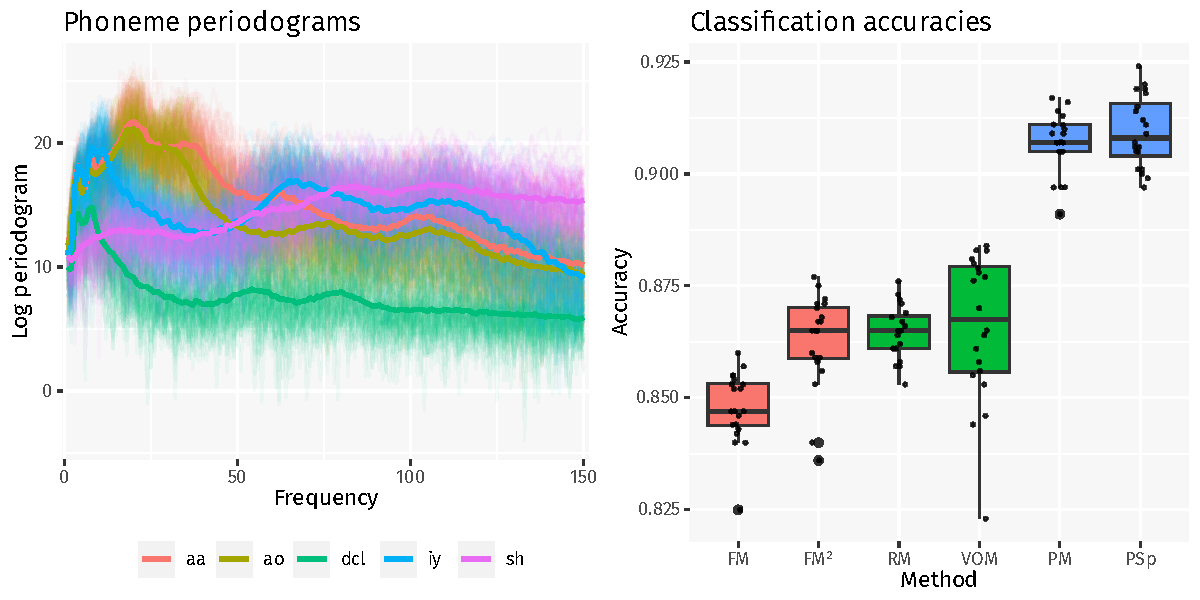
\includegraphics[width = \textwidth, page = 1]{phoneme}
    \caption{
        Classification of periodograms of digitized
        speech\protect\footnotemark, by phonemes (`aa', `ao', `dcl', `iy',
        `sh').
        The thick colored lines in the plot on the left mark the median curve
        across 400 examples in each of the five groups.
        The boxplot shows classification accuracies for 20 runs of each of the
        following methods: maximum depth classification using the first order
        (FM) and second order (FM$^2$) Fraiman-Muniz depths in red, the RM and
        VOM classifiers in green, and the maximum depth Mahalanobis (PM) and
        spatial (PSp) depth classifiers on $d$-variate feature vectors
        obtained by $d = 10$ random projections in blue.
        In each run, 50\% of the data was been aside for training.
    }
    \label{fig:phoneme_classification}
\end{figure}
\footnotetext{\url{http://www-stat.stanford.edu/ElemStatLearn}}



\subsection{Outlyingness matrices}

\textcite{dai-genton-2018} proposed a method which measures the outlyingness
of $\vx$ with respect to a population via depth as follows.

\begin{definition}
    Let $\vX$ be a $d$-variate stochastic process of continuous functions.
    At each time point $t \in [0, 1]$, the directional outlyingness is defined
    as
    \begin{equation}
        \vO(t) = \vO(\vX(t), F_{\vX(t)}) = \left(\frac{1}{D(\vX(t), F_{\vX(t)})} - 1\right)\, \vv(t),
    \end{equation}
    where $\vv(t)$ is the unit vector pointing from the median of $F_{\vX(t)}$
    to $\vX(t)$.
\end{definition}

\begin{definition}
    The functional directional outlyingness is defined as
    \begin{equation}
        \FO(\vX, F_{\vX}) = \int_{[0, 1]} \norm{\vO(t)}^2 \:w(t)\:dt.
    \end{equation}
\end{definition}

\begin{definition}
    \label{def:MO}
    The mean directional outlyingness is defined as
    \begin{equation}
        \MO(\vX, F_{\vX}) = \int_{[0, 1]} \vO(t) \:w(t)\:dt.
    \end{equation}
\end{definition}

\begin{definition}
    The variation of directional outlyingness is defined as
    \begin{equation}
        \VO(\vX, F_{\vX}) = \int_{[0, 1]} \norm{\vO(t) - \MO(t)}^2 \:w(t)\:dt.
    \end{equation}
\end{definition}

Here, $w$ is a weight function on $[0, 1]$.
In our discussion, we set $w = 1$.

It is easily verified that
\begin{equation}
    \FO^2 = \norm{\MO}^2 + \VO.
\end{equation}

\textcite{dai-genton-2018} propose using the $(d + 1)$-variate feature vectors
\begin{equation}
    \vY(\vX, F_{\vX}) = (\MO^\top,\, \VO)^\top
\end{equation}
corresponding to the curve $\vX$ for the purposes of classification.
The $\MO$ gives a sense of how outlying the curve $\vX$ is within $F_{\vX}$ as
a whole, while the $\VO$ measures the amount of variation in the outlyingness
over time.
Loosely speaking, $\MO$ is affected by the position, while $\VO$ is affected
by the shape of $\vX$ within $F_{\vX}$.
For instance, one may define the classifier
\begin{equation}
    \hat{\iota}(\vX) = \argmax_{1 \leq i \leq k} D'(\vY(\vX, F_i), F_{\vY(\vX, F_i)}),
\end{equation}
where $D'$ is a multivariate depth function.
This is simply a maximum depth classifier applied on the feature vectors
$\vY$.
When $D'$ is chosen to be the robust Mahalanobis depth, we have the RM
classifier
\begin{equation}
    \hat{\iota}_{RM}(\vX) = \argmax_{1 \leq i \leq k} D_{RM}(\vY(\vX, F_i), F_{\vY(\vX, F_i)}).
\end{equation}


\begin{definition}
    The functional directional outlyingness matrix is defined as
    \begin{equation}
        \FOM(\vX, F_{\vX}) = \int_{[0, 1]} \vO(t)\,\vO(t)^\top \:w(t)\:dt.
    \end{equation}
\end{definition}

\begin{definition}
    The functional directional outlyingness matrix is defined as
    \begin{equation}
        \VOM(\vX, F_{\vX}) = \int_{[0, 1]} (\vO(t) - \MO(t))\,(\vO(t) - \MO(t))^\top \:w(t)\:dt.
    \end{equation}
\end{definition}

Again, it is easily verified that
\begin{equation}
    \FOM = \MO\,\MO^\top + \VOM,
\end{equation}
and that
\begin{equation}
    \FO = \tr(\FOM), \qquad
    \VO = \tr(\VOM).
\end{equation}

We may also use the feature matrix $\VOM$, or its matrix norm $\norm{\VOM}_F$
corresponding to the curve $\vX$ for the purposes of classification.
Here, $\norm{\Cdot}_F$ denotes the Frobenius norm.
For instance, a $\VOM$ based classifier may be defined as
\begin{equation}
    \hat{\iota}_{\VOM}(\vX) = \argmin_{1 \leq i \leq k} \norm{\VOM(\vX, F_i)}_F.
\end{equation}



\subsection{Random projections}

Another approach is to use a feature vector consisting of multiple projections
of $\vX$.
Given functions $\vv_1, \dots, \vv_d$ chosen at random, we examine the
$d$-variate feature vectors
\begin{equation}
    \bm{V}(\vX, F_{\vX}) = \left(\ip{\vv_1}{\vX}, \dots, \ip{\vv_d}{\vX}\right)
\end{equation}
and apply a depth based multivariate classifier.
For instance, given a multivariate depth function $D'$, we may define a
classifier
\begin{equation}
    \hat{\iota}^d_{D'}(\vX) = \argmax_{1 \leq i \leq k} D'(\bm{V}(\vX, F_i), F_{\bm{V}(\vX, F_i)}).
\end{equation}


\section{Outlier detection}

\begin{figure}
    \centering
    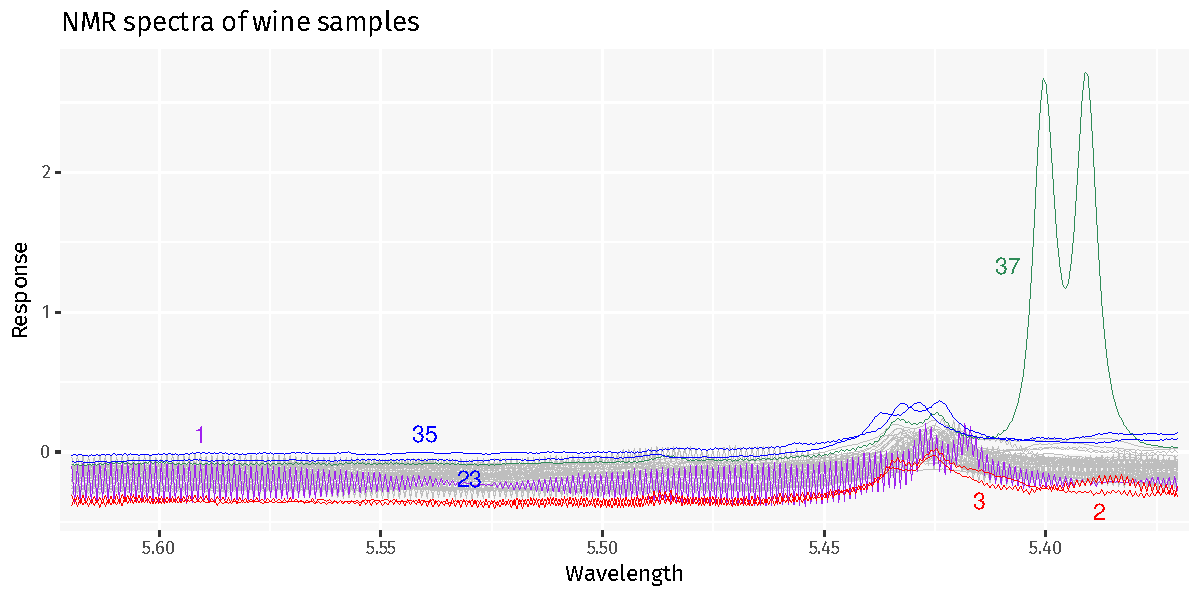
\includegraphics[width = \textwidth]{wine}
    \caption{
        NMR spectra of 40 wine samples, from the R package \texttt{speaq},
        with some curves showing outlying behaviour highlighted.
        The green curve \#37 is an isolated outlier, the blue and red curves
        are shift outliers, and the purple curve is a shape outlier.
    }
    \label{fig:wine}
\end{figure}

A curve $\vx\colon [0, 1] \to \R$ may exhibit outlying behaviour with respect
to a body of curves in many ways; we use the useful classification as detailed
in \textcite{hubert-rousseeuw-segeart-2015}.
It may deviate significantly over a short interval, in which case we call it
an \emph{isolated outlier}.
Alternatively, it may deviate over a large, or perhaps even the whole
interval, in which case we call it a \emph{persistent outlier}.
If this deviation is in terms of shape -- for instance, the curve may be
rougher or smoother -- we call it a \emph{shape outlier}.
Otherwise, if the curve has the same shape as the rest but appears above or
below them, we call it a \emph{shift outlier}.
Another possibility is that the curve differs in scale, in which case we call
it an \emph{amplitude outlier}.

An important consideration when dealing with shape outliers is that each time
slice $\vx(t)$ may be fairly inconspicuous with respect to the marginal
$F_{\vX(t)}$.
Thus, it seems clear that a tool like the Fraiman-Muniz depth may succeed in
identifying shift or amplitude outliers, but fall short against shape
outliers.
In general, the basic algorithm of iteratively selecting curves with low
functional depth as outliers is often insufficient.

A common approach towards examining the shapes of curves in a dataset is to
bundle them with their derivatives.


\subsection{Outliergrams}

\begin{figure}
    \centering
    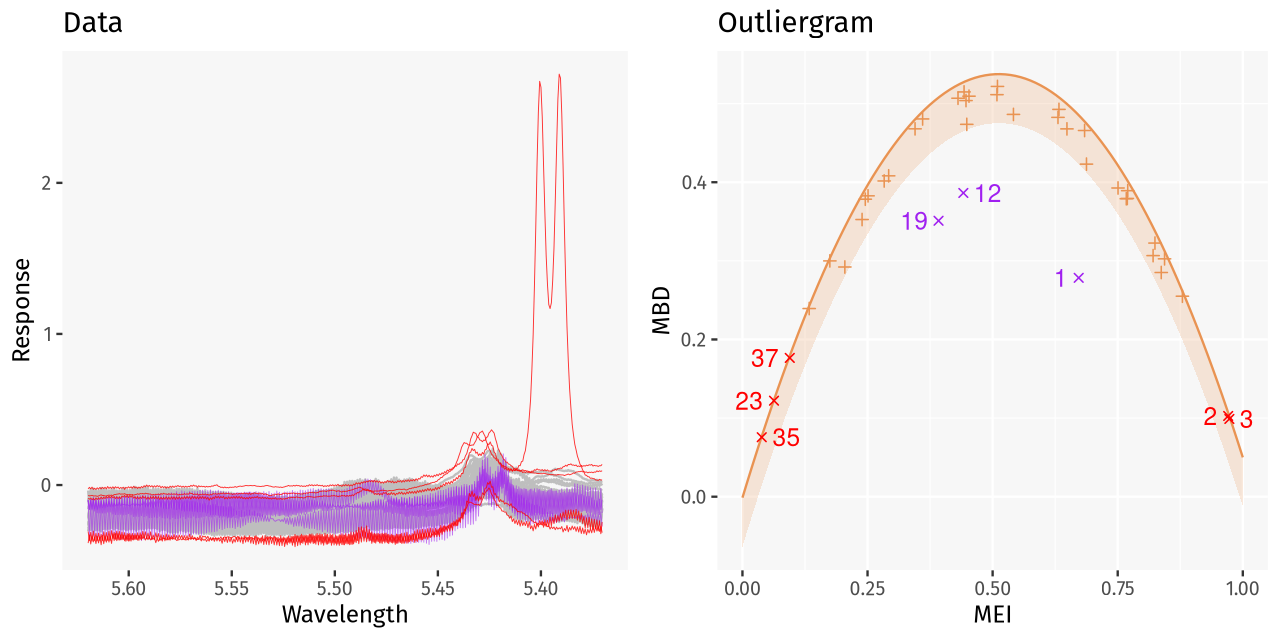
\includegraphics[width = \textwidth]{outliergram_wine}
    \caption{
        Outliergram for the NMR spectra of 40 wine samples.
        The three purple curves have been identified as shape outliers, as
        they fall outside the orange ribbon in the outliergram.
        Although the red curves lie on the orange parabola, they have low MBD
        and extreme MEI values, indicating that they lie above or below the
        main mass of curves.
    }
    \label{fig:outliergram_wine}
\end{figure}


\textcite{gil-romo-2014} combined the notions of the modified epigraph index
(MEI) and the modified band depth (MBD), proposing the outliergram as a tool
for detecting shape outliers.
They show that for a sample $\{\vx_i\}_{i = 1}^n$, each
\begin{equation}
    \MBD(\vx_i) = D_{MB}(\vx_i, \hat{F}_n) \leq a_0 + a_1 \MEI(\vx_i) + a_2 n^2 \MEI(\vx_i)^2
\end{equation}
where $a_0 = a_2 = -2/n(n - 1)$ and $a_1 = 2(n + 1)/(n - 1)$.
The distance
\begin{equation}
    d_i = a_0 + a_1 \MEI(\vx_i) + a_2 n^2 \MEI(\vx_i) - \MBD(\vx_i)
\end{equation}
is indicative of the outlyingness of $\vx_i$.
\textcite{gil-romo-2014} consider shape outlying curves as those for which
$d_i \geq d^* = Q_3 + 1.5\IQR$, where $Q_3$ and $\IQR$ are the third quartile
and the interquartile range of $\{d_i\}_{i = 1}^n$ respectively.

\begin{definition}[Outliergram]
    The outliergram for a dataset $\mathscr{D} = \{\vx_i\}_{i = 1}^n$ is the
    graph
    \begin{equation}
        \{(\MEI(\vx_i, \hat{F}_n),\, \MBD(\vx_i, \hat{F}_n))\colon 1 \leq i \leq n\}.
    \end{equation}
    Shape outliers are curves $\vx_i$ such that $(\MEI_i, \MBD_i)$ falls
    outside a ribbon of height $d^*$ under the parabola $a_0 + a_1 \MEI +
    a_2n^2\MEI^2$.
\end{definition}

Figure~\ref{fig:outliergram_wine} illustrates the use of the outliergram.
We have also highlighted curves with fairly low or high MEI values as shift
outliers; a low MEI value indicates that the curve lies above the main mass of
curves, and a high MEI indicates that it lies below.


\subsection{Centrality-Stability diagrams}

\begin{figure}
    \centering
    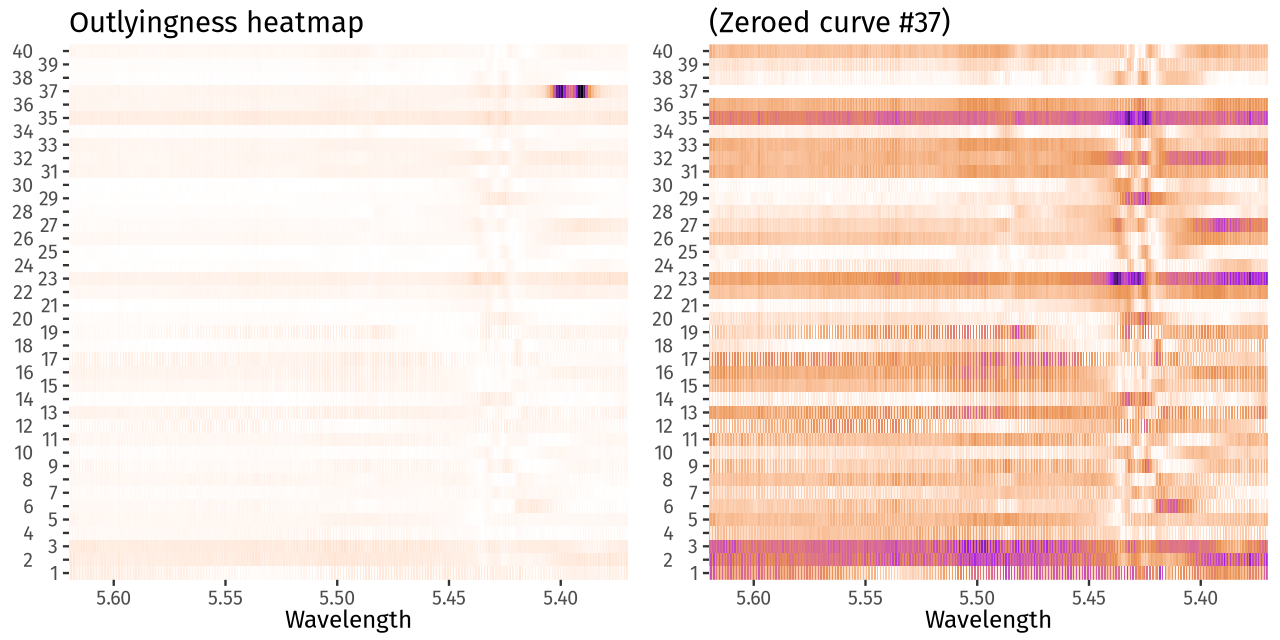
\includegraphics[width = \textwidth]{outlyingness_heatmap_wine}
    \caption{
        Outlyingness heatmap for the NMR spectra of 40 wine samples.
        The extreme curve \#37 has been zeroed out in the second diagram to
        better illustrate the variation in outlyingness for the remaining
        curves.
    }
    \label{fig:outlyingness_heatmap_wine}
\end{figure}

\begin{figure}
    \centering
    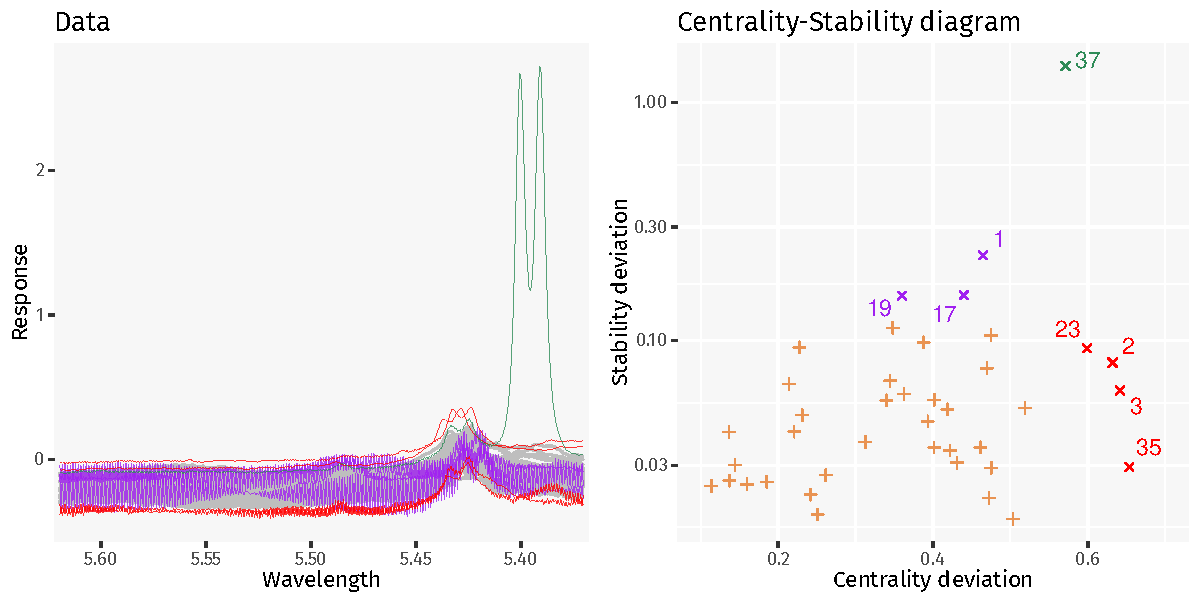
\includegraphics[width = \textwidth]{centrality_stability_wine}
    \caption{
        Centrality-Stability diagram for the NMR spectra of 40 wine samples.
        The red curves are seen to deviate in terms of centrality, indicated
        by the fact that the corresponding points in the centrality-stability
        diagram fall towards the right.
        The purple curves deviate in terms of stability, with the green curve
        showing extreme deviation.
    }
    \label{fig:centrality_stability_wine}
\end{figure}

In their discussion of methods of functional outlier detection,
\textcite{hubert-rousseeuw-segeart-2015} proposed the centrality-stability
diagram, where both the `centrality' of a curve (measured by depth) and its
variability in cross-sectional outlyingness over time are accounted for.
A deviation in centrality may point towards a shift outlier, while a deviation
in stability may point towards an isolated or shape outlier.

\textcite{hubert-rousseeuw-segeart-2015} begin by choosing a multivariate
depth function of the form $D'(\vx(t), F_{\vX(t)}) = (1 + O(\vx(t)))^{-1}$,
where $O(\Cdot)$ is an outlyingness function.
The Mahalanobis, projection, and Oja depths clearly fit this description.
Here, for the purposes of computation in the univariate case, we choose
\begin{equation}
    O(x(t)) = \frac{|x(t) - \med(X(t)|}{\MAD(X(t))},
\end{equation}
instead of using the skew-adjusted version; the differences are minor enough
for us to ignore.
The variation in $O(\vx(\Cdot))$ over time for different curves, in the form
of an \emph{outlyingess heatmap}, is quite revealing;
Figure~\ref{fig:outlyingness_heatmap_wine} shows that curves may have large
outlyingness for short or long intervals.

Corresponding to $D'$, we have an integrated Fraiman-Muniz depth
\begin{equation}
    D_F(\vx, F) = \int_{[0, 1]} (1 + O(\vx(t)))^{-1}\:dt.
\end{equation}
However, a spike in outlyingess over a short time interval, such as in curve
\#37 in Figure~\ref{fig:outlyingness_heatmap_wine}, may potentially be `washed
out' in this averaging.
With this, we seek a method of detecting sharp bursts in outlyingness.
Note that by setting
\begin{equation}
    \widetilde{\MOt}(\vx, F) = \int_{[0, 1]} O(\vx(t)) \:dt,% = \int_{[0, 1]} \left(\frac{1}{D'(\vx(t), F_{\vX(t)})} - 1\right) \:dt,
\end{equation}
Cauchy-Schwarz gives us the relation
\begin{equation}
    D_F(\vx, F) \Cdot (1 + \widetilde{\MOt}(\vx, F)) \geq 1.
\end{equation}
Equality is achieved only when $O(\vx(\Cdot))$ remains constant over time.
Any sudden variation in outlyingness over time will be detected by the
\emph{stability deviation}
\begin{equation}
    \Delta S(\vx, F) \;=\; (1 + \widetilde{\MOt}(\vx, F)) - \frac{1}{D_F(\vx, F)},
\end{equation}
the difference between the arithmetic and harmonic means of $1 +
O(\vx(\Cdot))$.
Defining the \emph{centrality deviation} simply as $\Delta C(\vx, F) = 1 -
D_F(\vx, F)$, we have our \emph{centrality-stability diagram}.

\begin{definition}[Centrality-Stability diagram]
    The centrality-stability diagram for a dataset $\mathscr{D} = \{\vx_i\}_{i
    = 1}^n$ is the graph
    \begin{equation}
        \{(\Delta C(\vx_i, \hat{F}_n),\, \Delta S(\vx_i, \hat{F}_n))\colon 1 \leq i \leq n\}.
    \end{equation}
\end{definition}

\begin{remark}
    We make a distinction between $\MO$ from Definition~\ref{def:MO} and
    $\widetilde{\MOt}$; the outlyingness $O(\Cdot)$ used in the latter is real
    and positive.
\end{remark}

Figure~\ref{fig:centrality_stability_wine} illustrates the use of the
centrality-stability diagram as a summary of the outlyingness heatmap from
Figure~\ref{fig:outlyingness_heatmap_wine}.
This time, the isolated outlier curve \#37 is well separated from the shift
and shape outliers, unlike in the outliergram in
Figure~\ref{fig:outliergram_wine}.




\subsection{MO-VO diagrams}

\begin{figure}
    \centering
    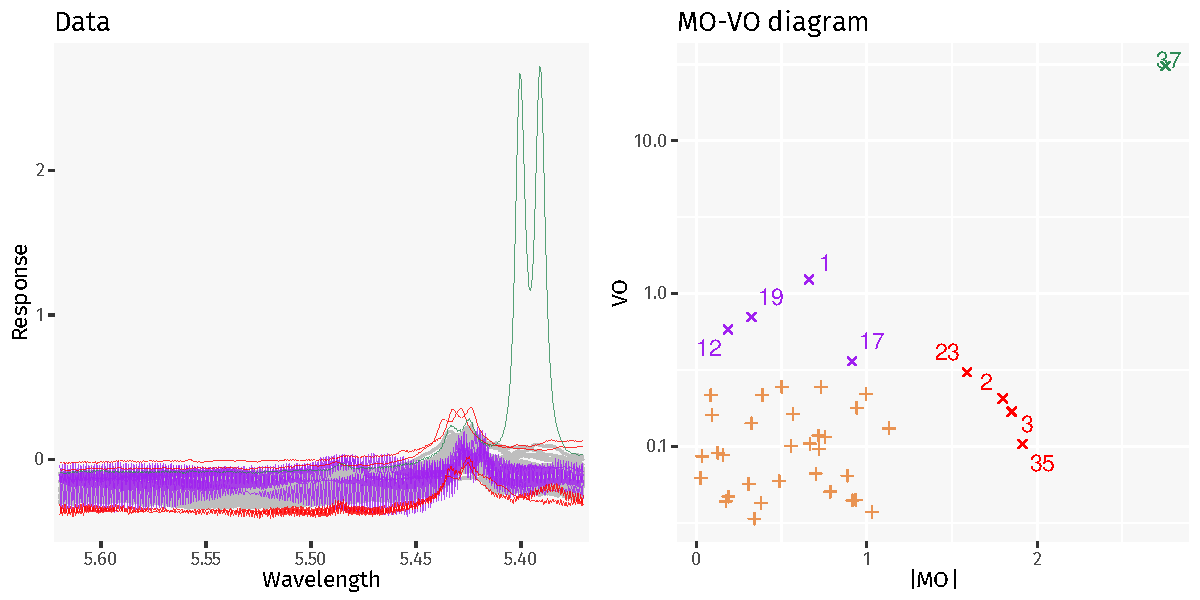
\includegraphics[width = \textwidth]{MO_VO_wine}
    \caption{
        MO-VO diagram for the NMR spectra of 40 wine samples.
        We plot $|\MOt|$ rather than MO here for better comparison with the
        centrality stability diagram in
        Figure~\ref{fig:centrality_stability_wine}; nevertheless, the signed
        MO values would reveal whether the shift outliers lie above or below
        the main mass of curves.
    }
    \label{fig:MO_VO_wine}
\end{figure}

We observe that the MO-VO diagram from \textcite{dai-genton-2018} neatly falls
under a general category of centrality-stability diagrams.
The quantity $\MO(\vx, F)$ may indeed be treated as a measure of deviation
from centrality of $\vx$.
Again, $\VO(\vx, F)$ being the variance of $\vO(t)$, may be treated as a
measure of deviation from stability, since it captures the variability of
outlyingness over time and is sensitive to changes over short intervals.

For the purposes of computation in the univariate case, we use the directional
outlyingess function
\begin{equation}
    O(x(t)) = \frac{x(t) - \med(X(t))}{\MAD(X(t))}.
\end{equation}
Figure~\ref{fig:MO_VO_wine} illustrates the use of the MO-VO diagram.
Note the similarities with the centrality-stability diagram from
Figure~\ref{fig:centrality_stability_wine}.




\begin{figure}
    \centering
    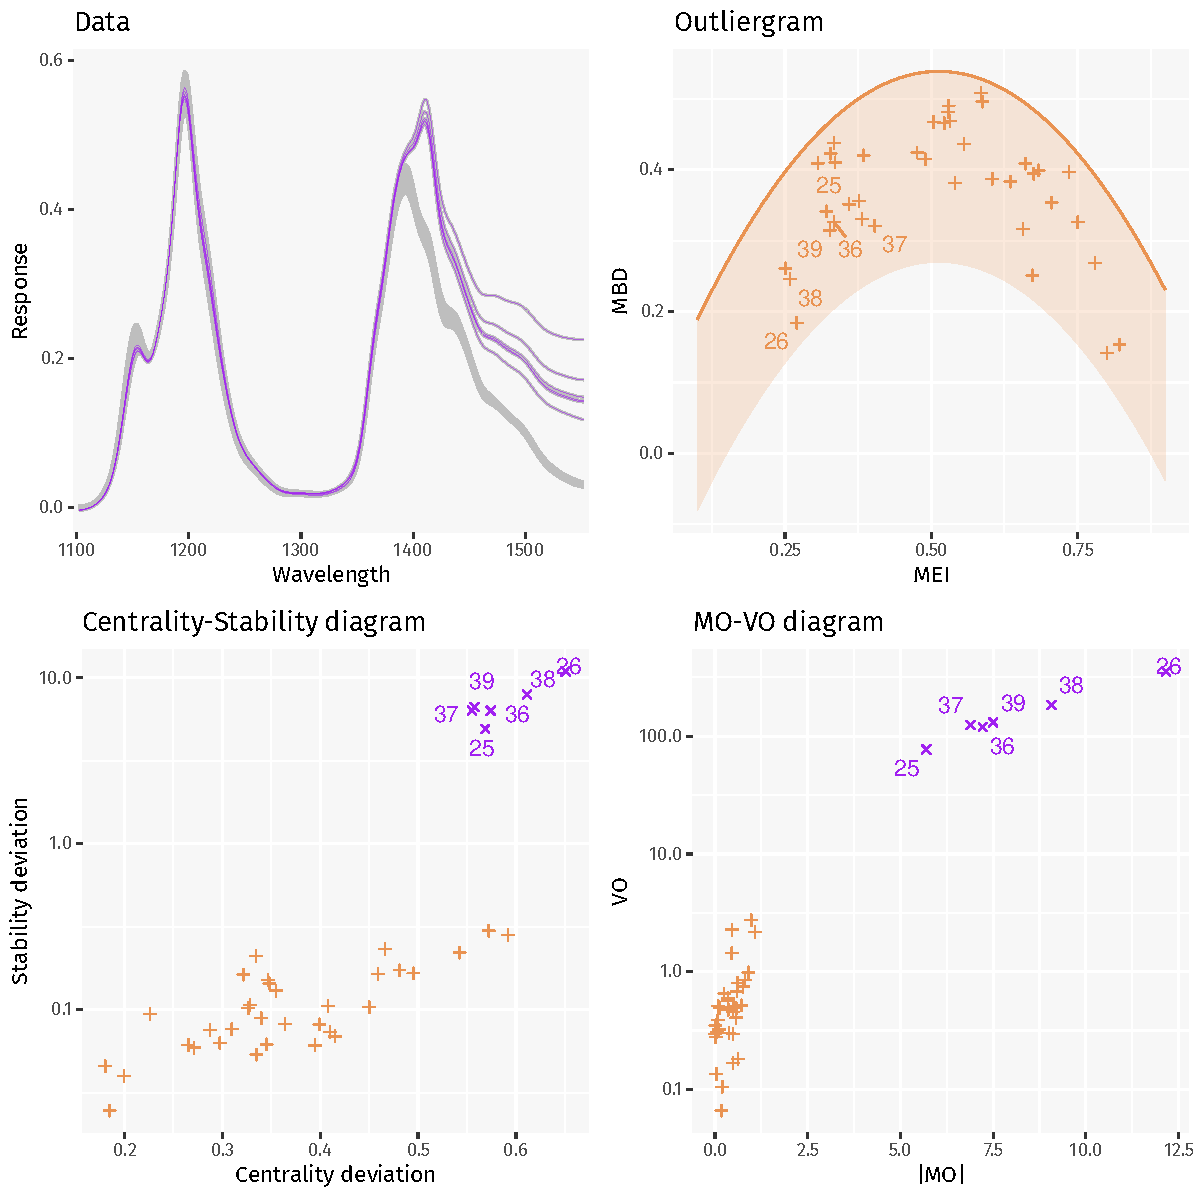
\includegraphics[width = \textwidth]{outlyingness_octane}
    \caption{
        Outliergram, centrality-stability, and MO-VO diagrams for the NIR
        spectra of 39 gasoline samples, from the R package \texttt{rrcov}.
        The six purple curves \#25, 26, 36-39 correspond to samples containing
        added alcohol.
        While the outliergram does not clearly identify these outliers, the
        centrality-stability and MO-VO diagrams show a marked separation from
        the main curves.
        Indeed, there is no cutoff $d^*$ defining the lower boundary of the
        orange ribbon in the outliergram which properly excludes the six
        outliers.
    }
    \label{fig:outlyingness_octane}
\end{figure}

\begin{figure}
    \centering
    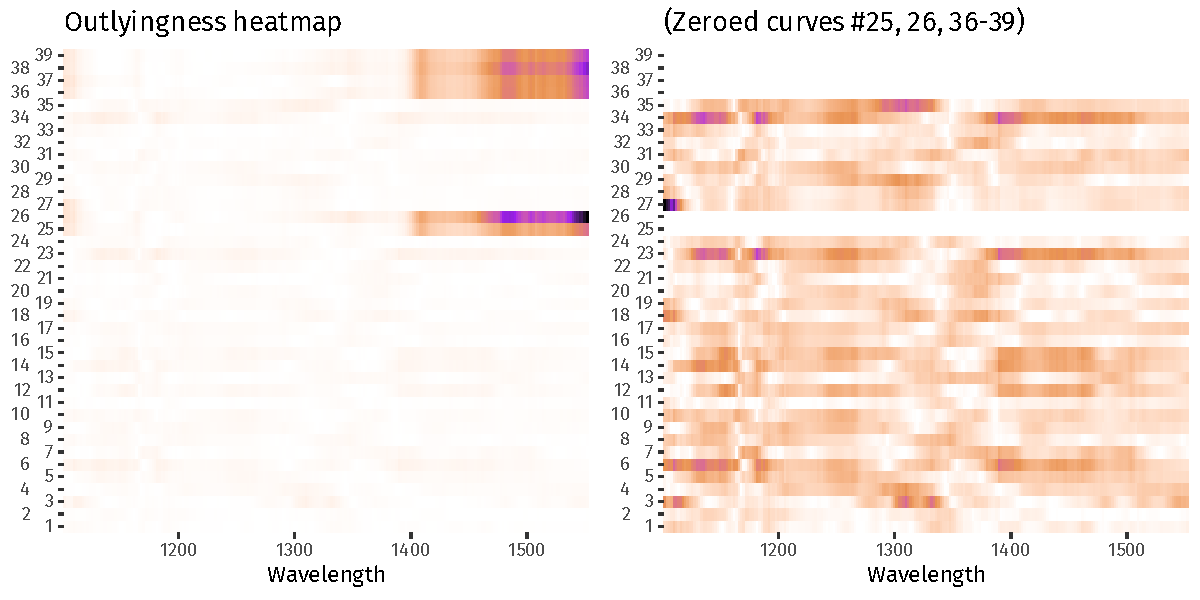
\includegraphics[width = \textwidth]{outlyingness_heatmap_octane}
    \caption{
        Outlyingness heatmap for the NIR spectra of 39 gasoline samples.
        The outlying curves have been zeroed out in the second diagram.
    }
    \label{fig:outlyingness_heatmap_octane}
\end{figure}


We use all of the above diagnostic tools on a different dataset in
Figures~\ref{fig:outlyingness_heatmap_octane} and \ref{fig:outlyingness_octane}.


% \section{Clustering}

\section{Partially observed functional data}

Consider the setting where the stochastic process $\vX$ of continuous
functions is not observed on the entire interval $[0, 1]$, but rather on a
random subset $O \subseteq [0, 1]$.
Then, a dataset of partially observed curves is of the form $\mathscr{D} =
\{(\vX_i, O_i)\}_{i = 1}^n$, where $\vX_i \iid F_{\vX}$, $O_i \iid Q$ where
$Q$ generates random compact subsets of $[0, 1]$, independent of $\vX_i$.
In other words, $(\vX_i, O_i) \iid F_{\vX} \times Q$.
This setup is known as the `Missing Completely at Random' assumption.

We set $\mathscr{J}(t) = \{j\colon t \in O_j\}$ to keep track of which curves
$\vX_i$ have been observed at time $t$.
Furthermore, denote $q(t) = |\mathscr{J}(t)|$ as the number of curves $\vX_i$
observed at time $t$.

\textcite{elias-jimenez-paganoni-sangalli-2023} propose the following.

\begin{definition}[Partially observed integrated functional depth]
    Let $D$ be a $d$-variate depth function.
    The Partially Observed Integrated Functional Depth (POIFD) is defined as
    \begin{equation}
        D_{POIFD}((\vx, o), F_{\vX} \times Q) = \int_o D(\vx(t), F_{\vX(t)})\:w_o(t) \:dt,
    \end{equation}
    where $w_o(t) = q(t) / \int_o q(t)\:dt$.
\end{definition}

We can now proceed with tasks such as classification, outlier detection, etc.\
on our partially observed dataset, via depth based procedures using POIFD
values.
Another natural problem is one of curve reconstruction: given a partially
observed curve $(\vX, O)$, can we estimate $\vX$ on $M = [0, 1]\setminus O$?

